\documentclass{article} % For LaTeX2e
\usepackage{iclr2027_conference,times}
\usepackage[table]{xcolor}

\usepackage{amsmath,amssymb,amsfonts}
\usepackage{booktabs}
\usepackage{graphicx}
\usepackage{multirow}
\usepackage{placeins}
\usepackage{microtype}
\usepackage{hyperref}
\usepackage{url}

\usepackage{tikz}
\usetikzlibrary{arrows.meta,calc,positioning}
\usepackage{pgfplots}
\pgfplotsset{compat=1.18}

\newcommand{\bx}{\mathbf{x}}
\newcommand{\bu}{\mathbf{u}}
\newcommand{\bt}{\mathbf{t}}
\newcommand{\R}{\mathbb{R}}
\newcommand{\E}{\mathbb{E}}
\newcommand{\Cin}{C_{\mathrm{in}}}
\newcommand{\Cout}{C_{\mathrm{out}}}
\newcommand{\code}[1]{\texttt{#1}}

% Per-column ranking shades: best / second / third.
\def\redc{\cellcolor[HTML]{FF999A}}
\def\orangec{\cellcolor[HTML]{FFCC99}}
\def\yellowc{\cellcolor[HTML]{FFF8AD}}
\newcommand{\ranklegend}{%
  \colorbox[HTML]{FF999A}{\strut\,best\,},
  \colorbox[HTML]{FFCC99}{\strut\,second\,}, and
  \colorbox[HTML]{FFF8AD}{\strut\,third\,}}

\emergencystretch=3em

\title{RBF-GNN: Rational Basis Functions for\\Pseudo-Coordinate based Graph Convolutions}

% Authors are hidden while \iclrfinalcopy is commented out;
% iclr2027_conference.sty substitutes the anonymous block for double-blind
% review.
\author{Anonymous authors \\
Paper under double-blind review}

%\iclrfinalcopy % Uncomment for camera-ready version, but NOT for submission.

\begin{document}

\maketitle

\begin{abstract}
We propose \ours{}, a new pseudo-coordinate based graph neural network architecture that takes into account euclidean, spherical or angular coordinates and uses them to induce a powerful spatial inductive bias.
Similar in architecture to SplineCNN, we improve upon the latter by replacing the less efficient sparse-activation based B-splines whose number grows exponentially with dimension by rational Pad\'e basis functions.
For effective training we propose a spline-subspace initialization and a variance-preserving weight rescaling. 
Experimentally, we evaluate on a number of popular neural network architectures that use SplineCNNs. We replace only the SplineCNNs with \ours{}.
We achieve improved results, including on semantic keypoint matching, shape matching, event based camera computer vision tasks.
We will make our implementation publicly available upon acceptance of the paper.
\end{abstract}


\section{Introduction}
\label{sec:intro}

Graph neural networks (GNN) encode geometric relationships between points. 
For graphs embedded in some coordinate space, for example Euclidean or spherical ones, SplineCNNs~\cite{fey2018splinecnn} are one of the best-performing methods that make explicit use of coordinates and enable higher performance than coordinate-free GNNs.
In particular, SplineCNN's coordinate-based convolution allows for efficient spatial localization and encodes a powerful inductive spatial bias.
Since many geometric tasks have relatively little data, this inductive bias is especially helpful.
This has resulted in SplineCNN being used, to our knowledge, in all state of the art semantic keypoint matching methods~\cite{...} for geometry based feature refinement.

SplineCNN works by modulating convolutions based on the activations of spatially localized B-splines.
However, SplineCNN has a few drawbacks:
\begin{description}
    \item[Sparsity:] B-splines form a partition of unity and for every coordinate only a few of them become non-zero. Hence, most of the convolutions are not active. This in turn makes it difficult to become computationally efficient on GPUs and means that convolutions receive relatively sparse updates during backpropagation.
    \item[Efficiency:] In order to localize activations spatially with enough precision in high dimensions, a fine enough partition of unity must be employed, necessitating a large enough B-spline bases. The size of this B-splines basis grows exponentially with the dimension of the coordinate space.
\end{description}

We propose to improve SplineCNN's architecture by replacing splines by rational safe Pad\'e basis functions.
Their advantages are:
\begin{itemize}
    \item more flexible, learnable localization
    \item increase computational efficiency and decrease required parameter count since fewer activation functions are needed due to them not being zero at most places and
    \item better scaling to higher dimensions, since the size of a B-spline basis grows exponentially with the number of coordinate dimensions.
\end{itemize}

We also show empirically the advantages of \ours{}.
We outperform SplineCNN based architectures by swapping SplineCNN for \ours{} and leaving everything else the same on the following benchmarks:
\begin{itemize}
    \item Sparse keypoint matching on PascalVOC~\cite{} and SPair-71K~\cite{} with the Deep Graph Matching Consensus~\cite{} architecture as well as the more recent ...~\cite{}.
    \item Shape matching on FAUST~\cite{}.
    \item Event-based camera computer vision~\cite{}.
\end{itemize}

\section{Related work}
\label{sec:related}

\paragraph{Geometry-aware graph convolutions.}
Message-passing neural networks provide the general neighbourhood-aggregation
view~\citep{gilmer2017mpnn}, while spatial operators additionally condition
messages on edge geometry. ECC generates filters from edge attributes
\citep{simonovsky2017ecc}; MoNet applies Gaussian mixtures to
pseudo-coordinates~\citep{monti2017monet}; and FeaStNet learns
feature-dependent assignments to weight matrices~\citep{verma2018feastnet}.
Continuous filters have also been generated by neural networks for molecules
\citep{schutt2017schnet}, point clouds~\citep{wang2018pccnn,wu2019pointconv},
and general graphs equipped with positional encodings~\citep{ma2024ckgconv}.
Related point-cloud operators use Taylor-polynomial filters
\citep{xu2018spidercnn}, learnable kernel points~\citep{thomas2019kpconv},
geometry-conditioned weight banks~\citep{xu2021paconv}, or relative-position
attention~\citep{zhao2021pointtransformer}. SplineCNN instead expands a
continuous kernel in compactly supported tensor-product B-splines
\citep{fey2018splinecnn}, an operator subsequently used for graph matching
\citep{fey2020dgmc} and event streams~\citep{schaefer2022aegnn}. RBF-GNN is
closest to SplineCNN: it preserves its message-passing rule and matrix bank,
but replaces the fixed grid basis by learnable non-separable rational
functions whose number is independent of $k^D$.

\paragraph{Learned continuous and rational bases.}
Learnable functional parameterisations include spline time--frequency atoms
\citep{balestriero2018splinefilters}, neural continuous kernels
\citep{romero2022ckconv,romero2022flexconv}, and coordinate networks based on
Fourier features, periodic activations, or multiplicative filters
\citep{tancik2020fourier,sitzmann2020siren,sahu2021mfn}. Rational functions
have been studied as trainable activations~\citep{molina2020pade} and as
efficient smooth approximators~\citep{boulle2020rational}. More recently, KAN
places learned B-spline functions on network edges~\citep{liu2025kan}, while
KAT replaces those splines by rational functions to improve efficiency and
scalability~\citep{yang2025kat}. Rational-activation and KAN-family models
modify neuron or feature-mixing nonlinearities, while neural coordinate models
learn an entire continuous signal or kernel. In contrast, our rational
functions are multivariate mixing coefficients of a matrix-valued graph kernel
and are initialised to preserve both the SplineCNN kernel subspace and its
output variance.


\begin{figure}[t]
\centering
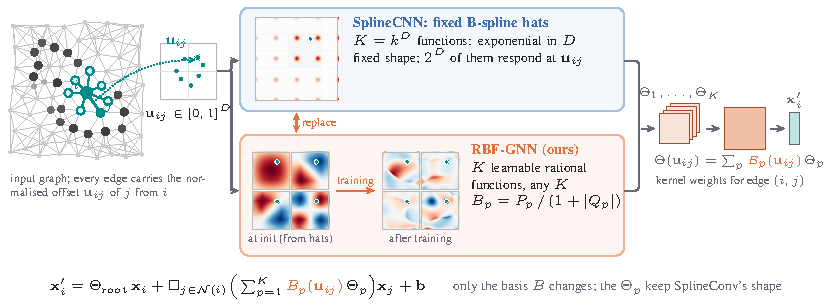
\includegraphics[width=\textwidth]{figures/method}
\caption{\textbf{RBF-GNN in one picture.} Every edge of the input graph
carries a pseudo-coordinate $\mathbf u_{ij}\in[0,1]^D$, the normalised offset
of $j$ from $i$. A continuous-kernel layer turns it into kernel weights
through a basis $B$, and this basis is the only thing we change: SplineCNN
uses $k^D$ fixed B-spline hats, RBF-GNN uses a small, freely chosen number of
learnable rational functions, initialised in the spline subspace and
reshaped by training (shown: the functions of one layer before and after
training on MNIST superpixels).}
\label{fig:method}
\end{figure}




\section{Method}
\label{sec:operator}

\ours{} is a graph convolution whose continuous kernel is spanned by learnable rational basis functions of pseudo-coordinates.
We first set up pseudo-coordinates and the continuous-kernel convolution operator, then introduce the rational basis in safe Pad\'e form.
A longer remark relates the construction to SplineCNN~\citep{fey2018splinecnn}, which uses the same operator with a fixed B-spline basis and for which \ours{} is a drop-in replacement.
Finally, we assemble the full network and describe the initialization that lets it train as reliably as the spline model it can replace.

\paragraph{Graphs and pseudo-coordinates.}
We consider graphs $G=(V,E)$ embedded in a coordinate space: every node $i$
carries features $\bx_i\in\R^{\Cin}$ and a spatial position $\bz_i\in\R^D$
(2-D image keypoints, vertices of a 3-D mesh, \dots). The convolution below
depends on \emph{relative} positions.
Because the kernel will be parameterised by basis functions living on a \emph{fixed, bounded}
domain, the offsets are affinely rescaled into the unit cube: with
$\delta_{\max}$ the largest absolute offset component occurring in the
graph, the \emph{pseudo-coordinate} of edge $(j,i)$ is
\begin{equation}
\bu_{ij} \;=\; \frac{\bz_j-\bz_i}{2\,\delta_{\max}} \;+\; \tfrac12\mathbf 1
\;\;\in\;[0,1]^D
\label{eq:pseudo}
\end{equation}
The zero offset lands at the centre $\tfrac12\mathbf 1$, a neighbour to the left/below has
$u_d<\tfrac12$ in that dimension, and the largest offset touches the
boundary.
See Figure~\ref{fig:coords} for an illustration of the pseudo-coordinate construction.
These pseudo-coordinates are the only way geometry enters the model. 
Polar or spherical encodings can be handled analoguously.

\paragraph{Continuous convolution kernels.}
An image convolution assigns a separate weight matrix to each of the
finitely many pixel offsets. On an irregular graph the offsets $\bu_{ij}$
vary continuously, so we instead learn a \emph{kernel function}
$g:[0,1]^D\to\R^{\Cin\times\Cout}$ and evaluate it at the observed
pseudo-coordinates. The kernel is parameterised as a linear combination
$g(\bu)=\sum_{p=1}^{K}B_p(\bu)\,\Theta_p$ of $K$ scalar basis
functions $B_p\colon[0,1]^D\to\R$ with learnable weight matrices
$\Theta_p\in\R^{\Cin\times\Cout}$, and a layer computes
\begin{equation}
\bx'_i \;=\; \Theta_{\mathrm{root}}\,\bx_i \;+\;
\mathop{\square}_{j\in\mathcal N(i)}\;\Bigl(\sum_{p=1}^{K} B_p(\bu_{ij})\,\Theta_p\Bigr)\bx_j \;+\; \mathbf b,
\label{eq:splineconv}
\end{equation}
with a separate root weight for the node itself, a bias, and aggregation
$\square \in \{\mathrm{mean}, \mathrm{add}\}$ over the neighbourhood.
This operator was introduced by SplineCNN~\citep{fey2018splinecnn}; the
difference lies entirely in the choice of the basis functions $B_p$, which
are fixed B-splines there (see the remark below) and learnable rational
functions here.

\begin{figure}[t]
\centering
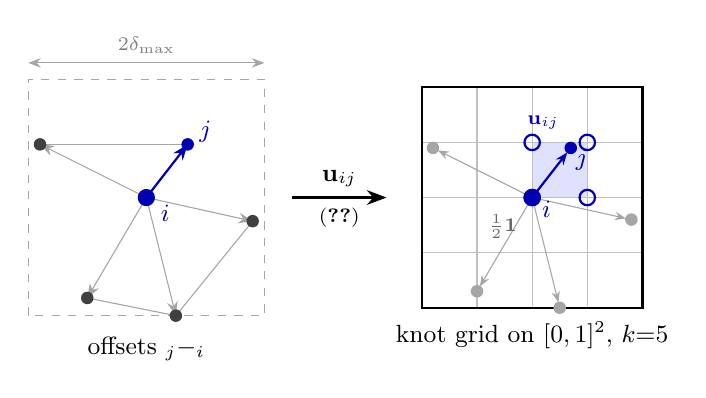
\begin{tikzpicture}[
  every node/.style={font=\small},
  vertex/.style={circle,fill=black!75,inner sep=1.6pt},
]
% ---- left: node i, its neighbours, and their offsets ----
% Offsets from i (delta_max = 1, attained by j5's second component):
%   j1 (-0.90, 0.45)   j2 ( 0.35, 0.45) <- highlighted edge
%   j3 ( 0.90,-0.20)   j4 (-0.50,-0.85)   j5 ( 0.25,-1.00)
% Right panel shows u = delta/(2*delta_max) + 1/2 of EXACTLY these offsets.
\begin{scope}[scale=1.5]
\coordinate (i)  at (0,0);
\coordinate (j1) at (-0.90,0.45);
\coordinate (j2) at (0.35,0.45);
\coordinate (j3) at (0.90,-0.20);
\coordinate (j4) at (-0.50,-0.85);
\coordinate (j5) at (0.25,-1.00);
% offset range that maps onto the unit square
\draw[dashed,gray!70] (-1,-1) rectangle (1,1);
\draw[{Stealth[length=1.6mm]}-{Stealth[length=1.6mm]},gray!70]
  (-1,1.14) -- (1,1.14) node[midway,above,gray,font=\scriptsize]
  {$2\delta_{\max}$};
% neighbour-neighbour edges (context only)
\draw[gray!70] (j1) -- (j2);
\draw[gray!70] (j3) -- (j5);
\draw[gray!70] (j4) -- (j5);
% offsets z_j - z_i as arrows out of i
\foreach \j in {j1,j3,j4,j5}
  \draw[-{Stealth[length=1.8mm]},gray!70] (i) -- (\j);
\draw[-{Stealth[length=2mm]},blue!70!black,thick] (i) -- (j2);
\foreach \j in {j1,j3,j4,j5} \node[vertex] at (\j) {};
\node[vertex,fill=blue!70!black] at (j2) {};
\node[blue!70!black] at ($(j2)+(0.15,0.11)$) {$j$};
\node[circle,fill=blue!70!black,inner sep=2.2pt] at (i) {};
\node[blue!70!black] at ($(i)+(0.16,-0.13)$) {$i$};
\node at (0,-1.28) {offsets $\bz_j-\bz_i$};
\end{scope}
% ---- mapping arrow ----
\draw[-{Stealth[length=2.5mm]},thick] (1.85,0) -- (3.05,0)
   node[midway,above] {$\bu_{ij}$}
   node[midway,below,font=\scriptsize] {\eqref{eq:pseudo}};
% ---- right: unit square with knot grid ----
% Same constellation, rescaled: u = delta/2 + 1/2.
\begin{scope}[shift={(3.5,-1.4)},scale=2.8]
  \fill[blue!12] (0.5,0.5) rectangle (0.75,0.75);
  \draw[step=0.25,gray!50,thin] (0,0) grid (1,1);
  \draw[thick] (0,0) rectangle (1,1);
  % centre = zero offset = image of node i; neighbours as on the left
  \coordinate (c) at (0.5,0.5);
  \foreach \p in {(0.05,0.725),(0.95,0.40),(0.25,0.075),(0.625,0.0)} {
     \draw[-{Stealth[length=1.4mm]},gray!70,shorten >=2pt] (c) -- \p;
     \node[vertex,fill=gray!70] at \p {};
  }
  \draw[-{Stealth[length=1.6mm]},blue!70!black,thick,shorten >=2pt]
    (c) -- (0.675,0.725);
  \node[vertex,fill=blue!70!black] (u) at (0.675,0.725) {};
  \node[blue!70!black] at ($(u)+(0.05,-0.055)$) {$j$};
  \node[blue!70!black,font=\scriptsize] at (0.55,0.84) {$\bu_{ij}$};
  \node[circle,fill=blue!70!black,inner sep=2.2pt] at (c) {};
  \node[blue!70!black] at ($(c)+(0.065,-0.055)$) {$i$};
  \node[font=\scriptsize,anchor=north east,black!60] at (0.475,0.465)
    {$\tfrac12\mathbf 1$};
  \foreach \p in {(0.5,0.5),(0.75,0.5),(0.5,0.75),(0.75,0.75)}
     \draw[blue!70!black,thick] \p circle (0.035);
  \node at (0.5,-0.125) {knot grid on $[0,1]^2$, $k{=}5$};
\end{scope}
\end{tikzpicture}
\caption{Pseudo-coordinates ($D{=}2$). \textbf{Left:} the
convolution at node $i$ sees each neighbour $j$ only through its spatial
offset $\bz_j-\bz_i$ (arrows); the dashed box marks the largest offset
magnitude $\delta_{\max}$ occurring in the graph. \textbf{Right:} the
shift-and-scale map \eqref{eq:pseudo} sends the dashed box to the unit
square, so the neighbourhood on the left reappears as a scaled copy: node
$i$ (zero offset) lands at the centre $\tfrac12\mathbf 1$, each neighbour
at its pseudo-coordinate --- $j$ at $\bu_{ij}$ (blue) --- and the largest
offset touches the boundary (bottom dot). The B-spline kernel is
defined once on this square via the $k{\times}k$ knot grid: at $\bu_{ij}$
only the $2^D{=}4$ hats anchored at the circled corners of the
containing cell (shaded) are non-zero, so only $4$ of the $K{=}25$ weight
matrices $\Theta_{\mathbf p}$ are used --- and updated --- for this edge.}
\label{fig:coords}
\end{figure}

\begin{figure}[t]
\centering
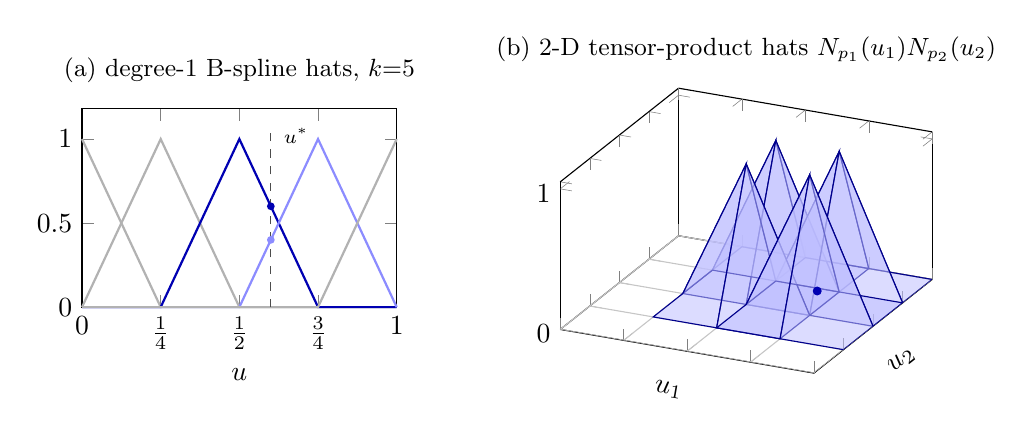
\begin{tikzpicture}
\begin{axis}[
  name=hats,
  width=0.46\linewidth, height=4.1cm,
  xmin=0, xmax=1, ymin=0, ymax=1.18,
  xtick={0,0.25,0.5,0.75,1},
  xticklabels={$0$,$\frac14$,$\frac12$,$\frac34$,$1$},
  ytick={0,0.5,1},
  xlabel={$u$},
  every axis plot/.append style={thick},
  title={\small (a) degree-1 B-spline hats, $k{=}5$},
  clip=false,
]
\addplot[gray!60] coordinates {(0,1) (0.25,0) (1,0)};
\addplot[gray!60] coordinates {(0,0) (0.25,1) (0.5,0) (1,0)};
\addplot[blue!70!black] coordinates {(0,0) (0.25,0) (0.5,1) (0.75,0) (1,0)};
\addplot[blue!45] coordinates {(0,0) (0.5,0) (0.75,1) (1,0)};
\addplot[gray!60] coordinates {(0,0) (0.75,0) (1,1)};
\draw[dashed,black!70] (axis cs:0.6,0) -- (axis cs:0.6,1.05);
\node[font=\scriptsize,anchor=west] at (axis cs:0.61,1.02) {$u^\ast$};
\fill[blue!70!black] (axis cs:0.6,0.6) circle (1.4pt);
\fill[blue!45]       (axis cs:0.6,0.4) circle (1.4pt);
\end{axis}
\begin{axis}[
  at={(hats.outer east)}, anchor=outer west, xshift=8mm,
  width=0.52\linewidth, height=5.2cm,
  view={25}{35},
  xmin=0, xmax=1, ymin=0, ymax=1, zmin=0, zmax=1.05,
  xtick={0,0.25,0.5,0.75,1}, ytick={0,0.25,0.5,0.75,1},
  xticklabels={,,,,}, yticklabels={,,,,}, ztick={0,1},
  xlabel={$u_1$}, ylabel={$u_2$},
  xlabel style={sloped}, ylabel style={sloped},
  title={\small (b) 2-D tensor-product hats $N_{p_1}(u_1)N_{p_2}(u_2)$},
  declare function={hat(\t,\c)=max(0,1-4*abs(\t-\c));},
]
% knot grid on the base plane
\foreach \x in {0,0.25,0.5,0.75,1} {
  \addplot3[gray!45, thin] coordinates {(\x,0,0) (\x,1,0)};
  \addplot3[gray!45, thin] coordinates {(0,\x,0) (1,\x,0)};
}
% the four pyramids active in the shaded cell of Fig.~\ref{fig:coords},
% painted back to front
\addplot3[surf, shader=flat, draw=blue!55!black, fill=blue!25,
          fill opacity=0.55, domain=0.25:0.75, y domain=0.5:1,
          samples=3, samples y=3] {hat(x,0.5)*hat(y,0.75)};
\addplot3[surf, shader=flat, draw=blue!55!black, fill=blue!25,
          fill opacity=0.55, domain=0.5:1, y domain=0.5:1,
          samples=3, samples y=3] {hat(x,0.75)*hat(y,0.75)};
\addplot3[surf, shader=flat, draw=blue!55!black, fill=blue!25,
          fill opacity=0.55, domain=0.25:0.75, y domain=0.25:0.75,
          samples=3, samples y=3] {hat(x,0.5)*hat(y,0.5)};
\addplot3[surf, shader=flat, draw=blue!55!black, fill=blue!25,
          fill opacity=0.55, domain=0.5:1, y domain=0.25:0.75,
          samples=3, samples y=3] {hat(x,0.75)*hat(y,0.5)};
% the pseudo-coordinate u_ij from Fig.~\ref{fig:coords}
\addplot3[only marks, mark=*, mark size=1.4pt, blue!70!black]
  coordinates {(0.675,0.725,0)};
\end{axis}
\end{tikzpicture}
\caption{The B-spline basis. \textbf{(a)} The five open degree-1 B-splines on
$[0,1]$; at any coordinate $u^\ast$ (dashed) only two are non-zero (dots), so
in $D$ dimensions only $2^D$ of the $k^D$ tensor products activate.
\textbf{(b)} 3-D view of the 2-D basis: each $B_{\mathbf p}$ is a pyramid
$N_{p_1}(u_1)N_{p_2}(u_2)$ centred on a knot pair. Shown are the four
pyramids anchored at the corners of the shaded cell of
Figure~\ref{fig:coords}; they are the only ones of the $K=k^2=25$ basis
functions that are non-zero at the pseudo-coordinate $\bu_{ij}$ (dot).}
\label{fig:bases}
\end{figure}

\paragraph{Rational safe Pad\'e basis functions.}
In \ours{} the scalar basis functions $B_p\colon[0,1]^D\to\R$ of \eqref{eq:splineconv} are learnable rational functions.
Each $B_p$ is a quotient of two polynomials whose coefficients are network parameters.
We build up the functional form in one dimension first.
A \emph{polynomial} of degree $m$ with learnable coefficients $a_0,\dots,a_m$ is
\begin{equation}
P(t) \;=\; \sum_{j=0}^{m} a_j\,t^j.
\label{eq:polynomial}
\end{equation}
A \emph{rational} function of degrees $(m,n)$ is a quotient of two such
polynomials,
\begin{equation}
R(t) \;=\; \frac{P(t)}{Q(t)}
\;=\; \frac{\sum_{j=0}^{m} a_j\,t^j}{\sum_{j=0}^{n} b_j\,t^j}.
\label{eq:rational}
\end{equation}
Training a free denominator is unstable, since it can become zero, making
the evaluation undefined, but also being close to zero will lead to numerical overflow.
We therefore use the \emph{safe} Pad\'e form~\citep{molina2020pade}, in which the denominator polynomial $Q$ (without constant term) enters only through $1+|Q(\cdot)|\ge 1$:
\begin{equation}
B(t) \;=\; \frac{P(t)}{1+\bigl|Q(t)\bigr|}
\;=\; \frac{\sum_{j=0}^{m} a_j\,t^j}
           {1+\Bigl|\sum_{j=1}^{n} b_j\,t^j\Bigr|},
\label{eq:safeform}
\end{equation}
which remains well defined and bounded for every value of the learnt coefficients $a_j,b_j$.
Figure~\ref{fig:pade} contrasts the plain rational~\eqref{eq:rational} with the safe form~\eqref{eq:safeform}.

In practice we expand $P$ and $Q$ not in the monomial basis $1,t,t^2,\dots$ but in Chebyshev polynomials of the first kind $\phi_0,\phi_1,\dots$ ($\phi_0{=}1$, $\phi_1{=}t$, $\phi_{j+1}{=}2t\phi_j-\phi_{j-1}$), i.e.\ $P(t)=\sum_j a_j\,\phi_j(t)$.
This parametrization spans the same function class but is better conditioned on bounded domains.
the map from monomial coefficients to polynomial values on an interval is exponentially ill-conditioned in the degree~\citep{gautschi1979condition}, so with monomials a small step in a high-order coefficient barely moves the function near $t=0$ but changes it violently near the boundary, giving gradients on wildly different scales.
The Chebyshev polynomials, by contrast, are orthogonal and uniformly bounded, $|\phi_j(t)|\le 1$ on $[-1,1]$, so every coefficient acts on a comparable scale and $|a_j|$ directly bounds the contribution of the $j$-th term; Chebyshev expansions are the standard well-conditioned representation of polynomials on bounded intervals in numerical practice~\citep{trefethen2019approximation}.

Below we extend this one-dimensional basis function to multiple dimensions in two different ways.

\begin{figure}[t]
\centering
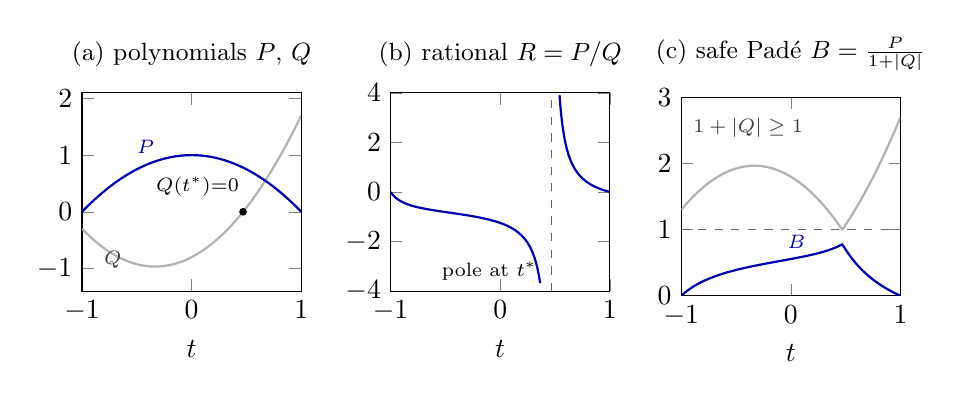
\begin{tikzpicture}[
  declare function={
    numP(\t)=1-\t*\t;
    denQ(\t)=1.5*\t*\t+\t-0.8;
  },
]
\begin{axis}[
  name=polys,
  width=0.36\linewidth, height=4.1cm,
  xmin=-1, xmax=1, ymin=-1.4, ymax=2.1,
  xtick={-1,0,1}, ytick={-1,0,1,2},
  xlabel={$t$},
  every axis plot/.append style={thick},
  title={\small (a) polynomials $P$, $Q$},
]
\addplot[gray!60, domain=-1:1, samples=100] {denQ(x)};
\addplot[blue!70!black, domain=-1:1, samples=100] {numP(x)};
\fill[black] (axis cs:0.4694,0) circle (1.4pt);
\node[font=\scriptsize, anchor=south east] at (axis cs:0.52,0.1)
  {$Q(t^\ast){=}0$};
\node[font=\scriptsize, blue!70!black] at (axis cs:-0.42,1.15) {$P$};
\node[font=\scriptsize, gray!45!black] at (axis cs:-0.72,-0.85) {$Q$};
\end{axis}
\begin{axis}[
  at={(polys.outer east)}, anchor=outer west, xshift=2mm,
  name=plainrat,
  width=0.36\linewidth, height=4.1cm,
  xmin=-1, xmax=1, ymin=-4, ymax=4,
  xtick={-1,0,1}, ytick={-4,-2,0,2,4},
  xlabel={$t$},
  every axis plot/.append style={thick},
  title={\small (b) rational $R=P/Q$},
]
\draw[dashed,black!60] (axis cs:0.4694,-4) -- (axis cs:0.4694,4);
\addplot[blue!70!black, domain=-1:0.45, samples=120,
  restrict y to domain=-4:4] {numP(x)/denQ(x)};
\addplot[blue!70!black, domain=0.49:1, samples=120,
  restrict y to domain=-4:4] {numP(x)/denQ(x)};
\node[font=\scriptsize, anchor=east] at (axis cs:0.42,-3.2)
  {pole at $t^\ast$};
\end{axis}
\begin{axis}[
  at={(plainrat.outer east)}, anchor=outer west, xshift=2mm,
  width=0.36\linewidth, height=4.1cm,
  xmin=-1, xmax=1, ymin=0, ymax=3,
  xtick={-1,0,1}, ytick={0,1,2,3},
  xlabel={$t$},
  every axis plot/.append style={thick},
  title={\small (c) safe Pad\'e $B=\frac{P}{1+|Q|}$},
]
\draw[dashed,black!60] (axis cs:-1,1) -- (axis cs:1,1);
\addplot[gray!60, domain=-1:1, samples=200] {1+abs(denQ(x))};
\addplot[blue!70!black, domain=-1:1, samples=200]
  {numP(x)/(1+abs(denQ(x)))};
\node[font=\scriptsize, gray!45!black, anchor=west] at (axis cs:-0.98,2.55)
  {$1+|Q|\ge 1$};
\node[font=\scriptsize, blue!70!black] at (axis cs:0.05,0.82) {$B$};
\end{axis}
\end{tikzpicture}
\caption{From polynomials to safe Pad\'e basis functions,
Eqs.~\eqref{eq:polynomial}--\eqref{eq:safeform}, with the same numerator
$P$ and denominator $Q$ in all three panels. \textbf{(a)}~Two polynomials
with learnable coefficients; $Q$ has a root $t^\ast$ inside the domain.
\textbf{(b)}~The plain rational function $R=P/Q$ diverges at $t^\ast$,
and any root of $Q$ can move into the domain during training.
\textbf{(c)}~In the safe form the denominator $1+|Q|$ (gray) never drops
below one (dashed), so $B$ stays bounded and well defined for every
setting of the coefficients; where $Q$ vanishes, $B$ simply equals $P$.}
\label{fig:pade}
\end{figure}

\paragraph{Product rational basis.}
Each of the $K$ basis functions factorises over the coordinate dimensions into univariate safe Pad\'e functions
\eqref{eq:safeform},
\begin{equation}
B_{\mathbf p}(\bu) \;=\; \prod_{d=1}^{D}
\frac{P_{d,p}(u_d)}{1+\bigl|Q_{d,p}(u_d)\bigr|},
\label{eq:safepade}
\end{equation}
where every factor has its own learnable polynomials $P_{d,p}$ and $Q_{d,p}$.

\paragraph{Multivariate rational basis.}
Each basis function $B_p\colon[0,1]^D\to\R$ is a single non-separable rational function of all coordinates jointly:
\begin{equation}
B_p(\bu) = \frac{P_p(\bu)}{1+|Q_p(\bu)|},\quad
P_p(\bu)=\!\!\sum_{|\alpha|\le m}\! a_{p,\alpha}\,
u_1^{\alpha_1}\!\cdots u_D^{\alpha_D},\quad
Q_p(\bu)=\!\!\sum_{1\le|\alpha|\le n}\! b_{p,\alpha}\,
u_1^{\alpha_1}\!\cdots u_D^{\alpha_D},
\label{eq:multivariate}
\end{equation}
with multi-indices $\alpha\in\mathbb N_0^D$ of total degree $|\alpha|\le m$ and $|\alpha|\le n$.
As in the univariate case, the implementation uses the Chebyshev parametrization.
Each monomial $u_1^{\alpha_1}\!\cdots u_D^{\alpha_D}$ is replaced by the product $\phi_{\alpha_1}(t_1)\cdots\phi_{\alpha_D}(t_D)$, spanning the same function class in better-conditioned form.

\paragraph{Original SplineCNN and B-spline basis.}
The original SplineCNN~\cite{fey2018splinecnn} uses the operator~\eqref{eq:splineconv}, but chooses the basis functions $B_p$ as B-splines, see Figure~\ref{fig:bases}.
This construction yields spatial localisation and a strong geometric inductive bias.
However, in every coordinate at most 2 B-splines are active, which means in larger dimensions that all but $2^D$ of the $\Theta_{\mathbf p}$ receive zero gradient.
This results in sparse, uneven updates and dense evaluation wasted on zeros.
The basis size $K=k^D$ grows exponentially with the coordinate dimension $D$ 


\paragraph{Initialization.}
Randomly initializing the basis functions works consistently worse.
We observe $-0.7$ to $-5.8$ drops in accuracy, see the ablation in our experiments.
Since we use small random numbers for initialization the resulting basis functions are approximately flat.
First, spatial localization would need to be completely learned from scratch.
Second, near-identical basis activations give the different $\Theta_p$ strongly correlated gradients.
Therefore, we propose two initializations that allow for spatial localization from the beginning.

\emph{Spline fit.}
Fit each rational function to its B-spline by least squares so the layer starts as approximately SplineConv.
We perform a stage-wise optimization to fit our learnable basis functions as follows:
\begin{enumerate}
    \item We fit the numerator $P$ with a closed-form least squares fit.
    \item Next, we refine both $P$ and $Q$ with Adam (lr $0.01$ for 500 steps.
    \item Last, for further numerical accuracy we use L-BFGS for 100 iterations on float64.
\end{enumerate}
We evaluate squared loss on a fixed grid of points, using 256 for 1D, $32^2$ for 2D and $16^2$ on 3D.
We use a small values for the denominator $Q$ since the gradient of a constant zero $Q$ would vanish.
The fit is cached, so stacked layers share the same fit.
The spline fit can be performed whenever the number of basis functions $K = k^d$ for some $k \in \N$. 

\emph{PCA of splines.} 
When $K \ne k^D$, we cannot fit to the splines.
Instead, we fit the $K$ functions to the $K$ leading principal components of the $k^D$ spline basis.
In detail, this is done as follows:
We sample points on the same grid as above.
We collect the values in a matrix $A$, compute its SVD and the the $K$ leading left singular vectors $u_1,\ldots,u_K$.
We rescale each $u_i$ to unit maximum and fix to a deterministic sign.
Last, we fit each $u_i$ with the same procedure as above for the spline fit.

\emph{Variance-preserving gain.}
The initialization of the kernel weights is calibrated for the spline basis.
The entries of $\Theta_p$ are drawn i.i.d.\ zero-mean with variance proportional to $1/(K\Cin)$ (\S\ref{sec:training}).
Thus, the message $\sum_p B_p(\bu)\,\Theta_p\,\bx_j$ along an edge has variance proportional to the basis energy $\sum_p B_p(\bu)^2$.
For partition-of-unity basis like the spline the variance remains.
However, the PCA-based initialization can result in larger activations and, without correction, to inflated output scale. 

Adapting a technique from KAT~\citep{yang2025kat}, we therefore rescale the
kernel weights by $\sqrt{\alpha}$ after basis initialization.
The gain compares the energy of the B-spline basis being replaced with that
of the initialized rational basis,
\begin{equation}
\alpha \;=\;
\E_{\bu}\Bigl[\sum_{\mathbf p} N_{\mathbf p}(\bu)^2\Bigr] \Big/\;
\E_{\bu}\Bigl[\sum_p B_p(\bu)^2\Bigr],
\label{eq:vp}
\end{equation}
where $N_{\mathbf p}$ are the $k^D$ tensor-product B-spline hats of
Figure~\ref{fig:bases}, $B_p$ are our $K$ rational basis functions as
returned by the spline or PCA fit above, and both expectations are over
uniform $\bu$, evaluated on the fit grid.
The initial message variance then matches that of SplineConv with the same
$K$.

\paragraph{Efficient implementation.}
A naive implementation of \ours{} materialises the Chebyshev feature tensor before contracting it with the coefficients.
More efficiently, we provide a triton kernel that never materializes this intermediate tensor that directly produces only $K$ basis values from the $D$ pseudo-coordinates.
The polynomial sums are efficiently computed by a Horner-like scheme.
The resulting kernel runs about $15x$ times faster than the naive  PyTorch implementation and $3x$ faster than a compiled variant and consumes less memory.
Training and inference with the Triton kernel for \ours{} is slightly faster overall than the PyG-implementation of SplineCNN.

\section{Experiments}
\label{sec:experiments}


\paragraph{Methods}
\begin{description}
    \item[\texttt{SplineCNN}:]
    \item[\texttt{MLP}:]
    \item[\texttt{\ours{}-uv}:]
    \item[\texttt{\ours{}-mv}:]
\end{description}

\paragraph{Keypoint matching on PascalVOC and SPair-71k.}
\label{sec:pascalvoc}
We evaluate semantic keypoint matching in two host pipelines that both use a
continuous-kernel graph convolution for geometric feature refinement: DGMC
\citep{fey2020dgmc} and NMT. In each pipeline we replace only the SplineConv
layers and leave the rest of the architecture, the backbone and the training
recipe untouched. Table~\ref{tab:keypoint} reports every configuration in both
pipelines on PascalVOC-Keypoints and SPair-71k.

\begin{table}[ht]
\centering\footnotesize
\setlength{\tabcolsep}{4pt}
\renewcommand{\arraystretch}{1.08}
\resizebox{\ifdim\width>\textwidth\textwidth\else\width\fi}{!}{%
\begin{tabular}{@{}lrrccrcc@{}}
\toprule
 & & \multicolumn{3}{c}{DGMC~\citep{fey2020dgmc}} & \multicolumn{3}{c}{NMT} \\
\cmidrule(lr){3-5}\cmidrule(lr){6-8}
Method & $K$ & Params $\downarrow$ & PascalVOC $\uparrow$ & SPair-71k $\uparrow$
       & Params $\downarrow$ & PascalVOC $\uparrow$ & SPair-71k $\uparrow$ \\
\midrule
\rowcolor[HTML]{EDEDED}
\multicolumn{8}{@{}l}{\textit{Spline baselines}} \\
SplineCNN & 25 & 9.50M & $73.00 \pm 0.40$ & $76.18 \pm 0.64$ & 28.17M & -- & \orangec $82.10 \pm 0.11$ \\
SplineCNN &  9 & 3.74M & $72.78 \pm 0.40$ & $76.04 \pm 0.43$ & 10.84M & -- & $81.54 \pm 0.31$ \\
SplineCNN &  4 & 1.93M & $71.48 \pm 0.40$ & $71.92 \pm 0.38$ &  5.42M & -- & $77.79 \pm 0.40$ \\
\rowcolor[HTML]{EDEDED}
\multicolumn{8}{@{}l}{\textit{MLP learned-basis control}} \\
MLP basis &  4 & 1.94M & $72.76 \pm 0.27$ & $73.74 \pm 0.71$ &  5.42M & -- & $80.40 \pm 0.57$ \\
MLP basis &  9 & 3.74M & $72.04 \pm 0.73$ & $74.34 \pm 0.62$ & 10.84M & -- & $81.05 \pm 0.32$ \\
\rowcolor[HTML]{EDEDED}
\multicolumn{8}{@{}l}{\textit{RBF-GNN with a product basis}} \\
\textbf{RBF-GNN} (product) & 25 & 9.50M & $72.88 \pm 0.48$ & $76.34 \pm 0.42$ & 28.17M & -- & \yellowc $82.08 \pm 0.21$ \\
\textbf{RBF-GNN} (product) &  9 & 3.74M & $73.26 \pm 0.18$ & $76.24 \pm 0.73$ & 10.84M & -- & $81.64 \pm 0.35$ \\
\rowcolor[HTML]{EDEDED}
\multicolumn{8}{@{}l}{\textit{RBF-GNN with a multivariate basis}} \\
\textbf{RBF-GNN} (mv), hat init &  9 & 3.74M & \redc $74.12 \pm 0.48$ & \orangec $77.68 \pm 0.35$ & 10.84M & -- & \redc $82.11 \pm 0.35$ \\
\textbf{RBF-GNN} (mv), PCA$+$vp &  4 & 1.94M & \yellowc $73.78 \pm 0.41$ & $77.44 \pm 0.36$ &  5.42M & -- & $81.52 \pm 0.22$ \\
\textbf{RBF-GNN} (mv), PCA$+$vp &  6 & 2.66M & \orangec $74.06 \pm 0.37$ & \redc $77.80 \pm 0.66$ &  7.59M & -- & $81.71 \pm 0.18$ \\
\textbf{RBF-GNN} (mv), PCA$+$vp &  9 & 3.74M & $73.72 \pm 0.19$ & \yellowc $77.50 \pm 0.27$ & 10.84M & -- & $81.59 \pm 0.14$ \\
\textbf{RBF-GNN} (mv), PCA$+$vp & 16 & 6.26M & $73.26 \pm 0.42$ & $77.14 \pm 0.40$ & 18.42M & -- & $81.69 \pm 0.27$ \\
\textbf{RBF-GNN} (mv), PCA$+$vp &  2 & 1.21M & $71.76 \pm 0.45$ & -- & -- & -- & -- \\
\textbf{RBF-GNN} (mv), PCA$+$vp &  1 & 0.85M & $68.26 \pm 0.36$ & -- & -- & -- & -- \\
\rowcolor[HTML]{EDEDED}
\multicolumn{8}{@{}l}{\textit{RBF-GNN degree control}} \\
\textbf{RBF-GNN} (mv $(5,4)$) & 25 & 9.51M & $73.08 \pm 0.25$ & $76.26 \pm 0.23$ & 28.17M & -- & $82.01 \pm 0.21$ \\
\bottomrule
\end{tabular}}
\caption{Semantic keypoint matching in two host pipelines. Accuracy (\%) is
mean $\pm$ std over 5 seeds; \ranklegend{} mark the three highest means
\emph{within each benchmark column}. $K$ is the number of basis functions and
is shared by both pipelines; the DGMC parameter counts are whole-model totals,
whereas the NMT counts cover the graph-convolution stack only and exclude the
frozen VGG16 backbone, so the two parameter columns are not comparable to each
other. Metrics follow each pipeline's own protocol and are likewise not
comparable across columns: DGMC/PascalVOC is averaged over the 20 object
categories, DGMC/SPair-71k is pair-averaged over 18 categories, and
NMT/SPair-71k is keypoint accuracy over 18 classes. Only SPair-71k under DGMC
has a validation split, so its column reports the validation-selected
checkpoint; the remaining columns report the best test epoch. Entries marked
``--'' were not run: NMT has no PascalVOC runs, and $K \in \{1,2\}$ was swept
on DGMC/PascalVOC only.}
\label{tab:keypoint}
\end{table}
\FloatBarrier

The multivariate rational basis is the strongest configuration in all three
populated columns. Its margin over the best spline baseline shrinks as the
host pipeline strengthens --- $+1.12$ on DGMC/PascalVOC, $+1.62$ on
DGMC/SPair-71k and $+0.01$ on NMT/SPair-71k --- so the accuracy gain is
pipeline-dependent. The margin over the MLP learned-basis control does not
follow that pattern ($+1.36$, $+3.46$ and $+1.06$), which indicates that the
structured rational form matters beyond merely learning the basis. The
parameter-efficiency result is the more robust one: a multivariate basis
matches or exceeds the widest spline grid in every column while using
$2.6$--$4.9\times$ fewer parameters. At matched $K$ the advantage is
concentrated at small bases ($+0.6$ to $+5.5$ for $K \in \{4,9\}$) and
vanishes at $K{=}25$.

\paragraph{Shape correspondence on FAUST.}
\label{sec:faust}
We evaluate dense shape correspondence on FAUST following the SplineCNN
protocol~\citep{fey2018splinecnn}. The task assigns every vertex of a held-out
human mesh to a template vertex, and we report exact-match accuracy over three
random seeds.

\begin{table}[ht]
\centering\footnotesize
\setlength{\tabcolsep}{4pt}
\renewcommand{\arraystretch}{1.08}
\resizebox{\ifdim\width>\textwidth\textwidth\else\width\fi}{!}{%
\begin{tabular}{@{}lrrc@{}}
\toprule
Method & $K$ & Params $\downarrow$ & Final $\uparrow$ \\
\midrule
\rowcolor[HTML]{EDEDED}
\multicolumn{4}{@{}l}{\textit{Spline baselines}} \\
\emph{SplineCNN $k{=}5$ (published)} & 125 & 4.10M & \emph{99.20} \\
SplineCNN $k{=}5$, mean $+$ clip & 125 & 4.11M & $98.71 \pm 0.08$ \\
SplineCNN $k{=}5$, add $+$ clip & 125 & 4.11M & $97.23 \pm 0.51$ \\
SplineCNN $k{=}5$, add, no clip & 125 & 4.11M & $29.1 \pm 50.3$ \\
SplineCNN $k{=}3$ & 27 & 2.30M & $83.6 \pm 15.6$ \\
SplineCNN $k{=}2$ & 8 & \orangec 1.95M & $3.4 \pm 3.3$ \\
\rowcolor[HTML]{EDEDED}
\multicolumn{4}{@{}l}{\textit{MLP learned-basis control}} \\
MLP basis, $K{=}8$ & 8 & \yellowc 1.96M & $98.21 \pm 1.11$ \\
\rowcolor[HTML]{EDEDED}
\multicolumn{4}{@{}l}{\textit{RBF-GNN with a product basis}} \\
\textbf{RBF-GNN} (product), $k{=}3$ & 27 & 2.30M & \yellowc $99.24 \pm 0.08$ \\
\rowcolor[HTML]{EDEDED}
\multicolumn{4}{@{}l}{\textit{RBF-GNN with a multivariate basis}} \\
\textbf{RBF-GNN} (multivariate), $K{=}4$ & 4 & \redc 1.89M & \orangec $99.38 \pm 0.09$ \\
\textbf{RBF-GNN} (multivariate), $K{=}4$, mean aggr. & 4 & \redc 1.89M & $98.93 \pm 0.10$ \\
\textbf{RBF-GNN} (multivariate), $K{=}8$ & 8 & 1.97M & \redc $99.41 \pm 0.04$ \\
\textbf{RBF-GNN} (multivariate), $K{=}16$ & 16 & 2.13M & $70.4 \pm 25.2$ \\
\textbf{RBF-GNN} (multivariate), $K{=}27$ & 27 & 2.34M & $19.0 \pm 32.8$ \\
\bottomrule
\end{tabular}}
\caption{FAUST shape correspondence. Accuracy (\%) is reported as mean
$\pm$ std over 3 seeds; the published SplineCNN result is from
\citet{fey2018splinecnn}. \ranklegend{} mark the three highest accuracy means
and the three smallest parameter counts.}
\label{tab:faust}
\end{table}
\FloatBarrier

Small multivariate rational bases give the best and most stable results with
substantially fewer parameters than SplineCNN. Their degradation at larger
basis sizes points to fragile PCA initialization rather than insufficient
capacity.

\paragraph{Event-based object recognition on N-Caltech101.}
\label{sec:ncaltech101}
We evaluate multiclass object recognition on N-Caltech101
\citep{orchard2015converting} with the seven-layer AEGNN recognition network
\citep{schaefer2022aegnn}. Each event is a graph node with space-time
pseudo-coordinates; we replace only the SplineConv layers and report test
accuracy over three random seeds.

\begin{table}[ht]
\centering\footnotesize
\setlength{\tabcolsep}{5pt}
\renewcommand{\arraystretch}{1.08}
\begin{tabular}{@{}lccrc@{}}
\toprule
Method & $K$ & Aggr. & Params $\downarrow$ & Final $\uparrow$ \\
\midrule
\rowcolor[HTML]{EDEDED}
\multicolumn{5}{@{}l}{\textit{Spline baselines}} \\
SplineCNN $k{=}2$ & 8 & mean & \orangec 77.68k & $47.35 \pm 0.15$ \\
SplineCNN $k{=}2$ & 8 & max & \orangec 77.68k & \orangec $56.00 \pm 0.92$ \\
\rowcolor[HTML]{EDEDED}
\multicolumn{5}{@{}l}{\textit{PointNet learned-kernel control}} \\
PointNet & -- & max & \redc 55.68k & $54.99 \pm 0.84$ \\
\rowcolor[HTML]{EDEDED}
\multicolumn{5}{@{}l}{\textit{RBF-GNN with a multivariate basis}} \\
\textbf{RBF-GNN} (multivariate) & 8 & mean & \yellowc 91.57k & \yellowc $55.05 \pm 0.58$ \\
\textbf{RBF-GNN} (multivariate) & 8 & max & \yellowc 91.57k & \redc $57.55 \pm 0.42$ \\
\bottomrule
\end{tabular}
\caption{N-Caltech101 event-based object recognition with AEGNN. Models use
training augmentation and validation-based convergence; test accuracy (\%) is
mean $\pm$ std over 3 seeds. \ranklegend{} mark the three highest means and
the three smallest parameter counts.}
\label{tab:ncaltech101}
\end{table}
\FloatBarrier

RBF-GNN performs best with max aggregation and also improves substantially
over SplineCNN under matched mean aggregation. Its advantage under both
aggregation rules shows that the gain is not explained only by the
neighborhood reducer.

\paragraph{Event-based car recognition on N-Cars.}
\label{sec:ncars}
We evaluate binary car-versus-background recognition on the real-world N-Cars
dataset~\citep{sironi2018hats} with the same AEGNN architecture and replacement
protocol~\citep{schaefer2022aegnn}. We report test accuracy after training for
30 epochs, averaged over three random seeds.

\begin{table}[ht]
\centering\footnotesize
\setlength{\tabcolsep}{5pt}
\renewcommand{\arraystretch}{1.08}
\begin{tabular}{@{}lccrc@{}}
\toprule
Method & $K$ & Aggr. & Params $\downarrow$ & Final $\uparrow$ \\
\midrule
\rowcolor[HTML]{EDEDED}
\multicolumn{5}{@{}l}{\textit{Spline baselines}} \\
SplineCNN $k{=}2$ & 8 & mean & \yellowc 26.99k & $87.83 \pm 0.25$ \\
SplineCNN $k{=}2$ & 8 & max & \yellowc 26.99k & $89.81 \pm 0.27$ \\
\rowcolor[HTML]{EDEDED}
\multicolumn{5}{@{}l}{\textit{PointNet learned-kernel control}} \\
PointNet & -- & max & \redc 4.99k & $87.17 \pm 0.24$ \\
\rowcolor[HTML]{EDEDED}
\multicolumn{5}{@{}l}{\textit{RBF-GNN with a multivariate basis}} \\
\textbf{RBF-GNN} (multivariate) & 4 & mean & \orangec 21.10k & \yellowc $90.24 \pm 0.39$ \\
\textbf{RBF-GNN} (multivariate) & 8 & mean & 40.88k & \orangec $90.49 \pm 0.05$ \\
\textbf{RBF-GNN} (multivariate) & 8 & max & 40.88k & \redc $91.00 \pm 0.43$ \\
\bottomrule
\end{tabular}
\caption{N-Cars event-based car recognition with AEGNN. Test accuracy (\%) is
mean $\pm$ std over 3 seeds; \ranklegend{} mark the three highest means and
the three smallest parameter counts.}
\label{tab:ncars}
\end{table}
\FloatBarrier

RBF-GNN is strongest under both aggregation rules, and its mean-aggregation
variant outperforms the max-aggregation SplineCNN. The smaller RBF-GNN
configuration also improves accuracy while using fewer parameters than
SplineCNN.

\paragraph{Superpixel graph classification on MNIST.}
\label{sec:mnist-superpixels}
We evaluate graph classification on MNIST superpixels following the SplineCNN
protocol~\citep{fey2018splinecnn}. The network uses two continuous-kernel
convolution layers with 2-D Cartesian pseudo-coordinates, and we report test
accuracy over three random seeds.

\begin{table}[ht]
\centering\footnotesize
\setlength{\tabcolsep}{5pt}
\renewcommand{\arraystretch}{1.08}
\begin{tabular}{@{}lrrc@{}}
\toprule
Method & $K$ & Params $\downarrow$ & Final $\uparrow$ \\
\midrule
\rowcolor[HTML]{EDEDED}
\multicolumn{4}{@{}l}{\textit{Spline baselines}} \\
SplineCNN $k{=}5$ & 25 & 88.36k & $97.41 \pm 0.13$ \\
SplineCNN $k{=}3$ & 9 & 55.08k & $96.49 \pm 0.12$ \\
SplineCNN $k{=}2$ & 4 & \redc 44.68k & $94.83 \pm 0.11$ \\
\rowcolor[HTML]{EDEDED}
\multicolumn{4}{@{}l}{\textit{MLP learned-basis control}} \\
MLP basis, $K{=}4$ & 4 & \yellowc 45.59k & $97.23 \pm 0.11$ \\
\rowcolor[HTML]{EDEDED}
\multicolumn{4}{@{}l}{\textit{RBF-GNN with a multivariate basis}} \\
\textbf{RBF-GNN} (multivariate), PCA$+$vp, $K{=}4$ & 4 & \orangec 45.26k & \yellowc $97.79 \pm 0.08$ \\
\textbf{RBF-GNN} (multivariate), PCA$+$vp, $K{=}9$ & 9 & 56.38k & \redc $98.00 \pm 0.16$ \\
\textbf{RBF-GNN} (multivariate), hat init, $k{=}3$ & 9 & 56.38k & \orangec $97.87 \pm 0.06$ \\
\bottomrule
\end{tabular}
\caption{MNIST superpixel graph classification. Test accuracy (\%) is mean
$\pm$ std over 3 seeds; \ranklegend{} mark the three highest means and the
three smallest parameter counts.}
\label{tab:mnist-superpixels}
\end{table}
\FloatBarrier

RBF-GNN gives the three strongest results and improves over SplineCNN at both
matched and reduced basis sizes. Its advantage over the equal-width MLP
control supports the rational parameterization itself.

\paragraph{Superpixel graph classification on CIFAR-10 with 5-D bilateral
coordinates.}
\label{sec:cifar10-superpixels}
We evaluate CIFAR-10 superpixel graph classification from
GNNBenchmarkDataset~\citep{dwivedi2023benchmarking}. The bilateral
pseudo-coordinate concatenates relative 2-D centroid position and RGB
features into a 5-D kernel, and we report test accuracy over three random
seeds.

\begin{table}[ht]
\centering\footnotesize
\setlength{\tabcolsep}{5pt}
\renewcommand{\arraystretch}{1.08}
\begin{tabular}{@{}lrrc@{}}
\toprule
Method & $K$ & Params $\downarrow$ & Final $\uparrow$ \\
\midrule
\rowcolor[HTML]{EDEDED}
\multicolumn{4}{@{}l}{\textit{Spline baselines}} \\
SplineCNN $k{=}3$ & 243 & 557.42k & $58.73 \pm 0.26$ \\
SplineCNN $k{=}2$ & 32 & 105.03k & $57.55 \pm 0.34$ \\
\rowcolor[HTML]{EDEDED}
\multicolumn{4}{@{}l}{\textit{MLP learned-basis control}} \\
MLP basis, $K{=}8$ & 8 & \orangec 55.39k & \orangec $59.67 \pm 0.32$ \\
MLP basis, $K{=}32$ & 32 & \yellowc 109.96k & \yellowc $59.02 \pm 0.10$ \\
\rowcolor[HTML]{EDEDED}
\multicolumn{4}{@{}l}{\textit{RBF-GNN with a multivariate basis}} \\
\textbf{RBF-GNN} (multivariate), $K{=}4$ & 4 & \redc 46.45k & $57.58 \pm 0.23$ \\
\textbf{RBF-GNN} (multivariate), $K{=}8$ & 8 & \yellowc 56.47k & $58.97 \pm 0.16$ \\
\textbf{RBF-GNN} (multivariate), $K{=}32$ & 32 & 116.62k & \redc $59.87 \pm 0.40$ \\
\bottomrule
\end{tabular}
\caption{CIFAR-10 superpixel graph classification with 5-D bilateral
pseudo-coordinates. Test accuracy (\%) is mean $\pm$ std over 3 seeds;
\ranklegend{} mark the three highest means and the three smallest parameter
counts.}
\label{tab:cifar10-bilateral}
\end{table}
\FloatBarrier

RBF-GNN attains the best accuracy while using far fewer parameters than the
wider spline grid. The lower-width sweep remains competitive, although the
MLP control is strongest at the smallest shared width.

\paragraph{Part segmentation on ShapeNet-Part with 6-D coordinates.}
\label{sec:shapenet-part}
We evaluate point-cloud part segmentation on ShapeNet-Part~\citep{yi2016scalable}
using a fixed subset of 4,000 training and 1,333 test shapes. Relative
positions and surface normals define 6-D pseudo-coordinates on a
16-nearest-neighbor graph, and we report instance-average mIoU over three
random seeds.

\begin{table}[ht]
\centering\footnotesize
\setlength{\tabcolsep}{5pt}
\renewcommand{\arraystretch}{1.08}
\begin{tabular}{@{}lrrc@{}}
\toprule
Method & $K$ & Params $\downarrow$ & Final mIoU $\uparrow$ \\
\midrule
\rowcolor[HTML]{EDEDED}
\multicolumn{4}{@{}l}{\textit{Spline baselines}} \\
SplineCNN $k{=}3$ & 729 & 1.60M & \redc $65.12 \pm 0.41$ \\
SplineCNN $k{=}2$ & 64 & 177.91k & $60.02 \pm 0.23$ \\
\rowcolor[HTML]{EDEDED}
\multicolumn{4}{@{}l}{\textit{MLP learned-basis control}} \\
MLP basis, $K{=}8$ & 8 & \redc 60.75k & $62.80 \pm 0.45$ \\
MLP basis, $K{=}32$ & 32 & \yellowc 116.88k & \yellowc $63.81 \pm 0.46$ \\
\rowcolor[HTML]{EDEDED}
\multicolumn{4}{@{}l}{\textit{RBF-GNN with a multivariate basis}} \\
\textbf{RBF-GNN} (multivariate), $K{=}8$ & 8 & \orangec 64.87k & $61.88 \pm 0.38$ \\
\textbf{RBF-GNN} (multivariate), $K{=}32$ & 32 & 137.43k & \orangec $64.86 \pm 0.18$ \\
\bottomrule
\end{tabular}
\caption{ShapeNet-Part segmentation with 6-D position--normal
pseudo-coordinates. Instance-average mIoU (\%) is mean $\pm$ std over 3 seeds;
\ranklegend{} mark the three highest means and the three smallest parameter
counts.}
\label{tab:shapenet-part}
\end{table}
\FloatBarrier

RBF-GNN nearly matches the large spline grid with an order-of-magnitude
smaller model and outperforms the equal-width MLP control. At the narrowest
width the MLP is stronger, so this benchmark supports efficient scaling
rather than universal gains at every capacity.

\paragraph{Keypoint matching on WILLOW-ObjectClass.}
We evaluate semantic keypoint matching on WILLOW-ObjectClass with the DGMC
pipeline~\citep{fey2020dgmc}, without PascalVOC pretraining. We report final
matching accuracy over ten runs and include an initialization ablation for
the product rational basis.

\begin{table}[ht]
\centering\footnotesize
\setlength{\tabcolsep}{6pt}
\renewcommand{\arraystretch}{1.08}
\begin{tabular}{@{}lc@{}}
\toprule
Method & Final $\uparrow$ \\
\midrule
\rowcolor[HTML]{EDEDED}
\multicolumn{2}{@{}l}{\textit{Spline baselines}} \\
SplineCNN & $96.80 \pm 1.20$ \\
\rowcolor[HTML]{EDEDED}
\multicolumn{2}{@{}l}{\textit{RBF-GNN with a product basis}} \\
\textbf{RBF-GNN} (product), hat init & \yellowc $97.28 \pm 1.01$ \\
\textbf{RBF-GNN}, Gaussian init & \redc $97.72$ \\
\textbf{RBF-GNN}, Chebyshev$+$vp init & $97.07$ \\
\textbf{RBF-GNN}, random$+$vp init & $92.13$ \\
\textbf{RBF-GNN}, constant init & $10.00$ \\
\rowcolor[HTML]{EDEDED}
\multicolumn{2}{@{}l}{\textit{RBF-GNN with a multivariate basis}} \\
\textbf{RBF-GNN} (multivariate), $k{=}5$ & \orangec $97.55 \pm 0.63$ \\
\bottomrule
\end{tabular}
\caption{WILLOW-ObjectClass keypoint matching. Final accuracy (\%) is shown;
the backbone comparison reports mean $\pm$ std over 10 runs. \ranklegend{}
mark the three highest means.}
\label{tab:willow}
\end{table}
\FloatBarrier

The multivariate model gives the best mean accuracy, although the backbone
differences are not statistically significant. Initialization strongly
affects optimization, and a constant basis collapses to chance performance.

\paragraph{Keypoint matching on PascalPF.}
We evaluate semantic keypoint matching on synthetic and PascalPF image pairs
following DGMC~\citep{fey2020dgmc}. We report final matching accuracy over
three random seeds and compare the initialization strategies used for the
product rational basis.

\begin{table}[ht]
\centering\footnotesize
\setlength{\tabcolsep}{6pt}
\renewcommand{\arraystretch}{1.08}
\begin{tabular}{@{}lc@{}}
\toprule
Method & Final $\uparrow$ \\
\midrule
\rowcolor[HTML]{EDEDED}
\multicolumn{2}{@{}l}{\textit{Spline baselines}} \\
SplineCNN, $k{=}5$ & \yellowc $95.27 \pm 0.15$ \\
\rowcolor[HTML]{EDEDED}
\multicolumn{2}{@{}l}{\textit{RBF-GNN with a product basis}} \\
\textbf{RBF-GNN} (product), $k{=}3$, hat init & \orangec $95.73 \pm 0.06$ \\
\textbf{RBF-GNN}, Gaussian init & \redc $95.90$ \\
\textbf{RBF-GNN}, random init & $94.93$ \\
\textbf{RBF-GNN}, constant init (two variants) & $78$ / $66$ \\
\bottomrule
\end{tabular}
\caption{PascalPF keypoint matching. Final accuracy (\%) is reported as mean
$\pm$ std over 3 seeds where available. \ranklegend{} mark the three highest
means.}
\label{tab:pascalpf}
\end{table}
\FloatBarrier

The rational basis has higher mean accuracy than the spline baseline, although
the difference remains within seed variability. The poor constant
initialization again shows that a non-degenerate starting basis is essential.

% \section{Practical recipe}
% \label{sec:recipe}
%
% \begin{enumerate}
% \item Use the multivariate basis, total degrees $(8,6)$, safe-B, Chebyshev.
% \item Choose $K \approx 4$--$8$, independent of dimension.
% \item Init: hat-fit when $K=k^D$, else PCA-of-hats; always with the vp gain;
%   never a zero denominator.
% \item Train exactly like the SplineCNN you are replacing; add grad-norm
%   clipping for deep stacks with add-aggregation.
% \item Expect $\approx$ equal accuracy at ${\sim}2$--$5\times$ fewer
%   parameters, or $+0.7$--$1.8$ pts at equal parameter count; expect
%   10--40\% slower epochs.
% \end{enumerate}
%
% \section{Open questions / limitations}
% \label{sec:limitations}
%
% \begin{itemize}
% \item Large-$K$ PCA-init fragility in 3-D (localised targets for the higher
%   components should fix it).
% \item Basis-coefficient scale drift at large $K$ (safe-Pad\'e gauge freedom;
%   benign on accuracy, visible in parameter norms~/ calibration).
% \item Mean vs add aggregation interacts with the basis (mean helps spline,
%   mildly hurts rational on FAUST); unexplained.
% \item Timing uses a pure-PyTorch SplineConv baseline; against the CUDA
%   \code{torch-spline-conv} kernel the rational overhead would be larger.
% \item WILLOW/PascalPF gains are within seed noise; the significant results
%   are PascalVOC and FAUST.
% \end{itemize}

% ---------------------------------------------------------------------------
% ICLR 2027 end-of-main-text statements, placed before the references. The AI
% use statement is REQUIRED by the 2027 call; the ethics and reproducibility
% statements are recommended. None of the three counts toward the 9-page
% main-text limit.
% ---------------------------------------------------------------------------
\subsection*{AI use statement}

[TODO --- required by ICLR 2027. Disclose which generative AI tools were used
and for what.]

\subsection*{Ethics statement}

[TODO --- recommended.]

\subsection*{Reproducibility statement}

[TODO --- recommended. Point at the released code, the named configurations
in \code{slurm/configs.sh}, the per-run training logs under
\code{results/logs/}, and the fixed seeds used for each table.]

\bibliographystyle{iclr2027_conference}
\enlargethispage{2\baselineskip}
\bibliography{rational_basis}

\end{document}
